\documentclass{beamer}
\usepackage[utf8]{inputenc}
\usepackage[T1]{fontenc}
\usepackage[french]{babel}
\usepackage{graphicx}
\usepackage{amsmath}
\usepackage{amssymb}
\usepackage{hyperref}

\title{Présentation du prjets de programmation impérative}
\author{\textsc{Breuil} Dorian, \textsc{Defay} Adrien et \textsc{Peyrard} Gaultier}
\date{\today}

\begin{document}

\frame{\titlepage}  % Crée la première page avec le titre

\begin{frame}
  \frametitle{Table des matières}
  \tableofcontents
  
\end{frame}

\section{Introduction}
\begin{frame}
  \frametitle{Introdutions}  % Titre de la diapositive
  % Contenu de la diapositive
  Voici nos choix de pensées pour notre projet.
\end{frame}

\section{Choix de l'ia}
\begin{frame}
  \frametitle{Choix de l'ia}  % Titre de la diapositive
  % Contenu de la diapositive
  
\end{frame}

\section{Structure de données}
\begin{frame}
  \frametitle{Structure de données}
  \begin{itemize}
  \item Structure plateau.
  \item Structure arbre.
  \item Structure coordonnée.
  \end{itemize}
\end{frame}

\subsection{Structure plateau}
\begin{frame}
  \frametitle{Structure plateau}
  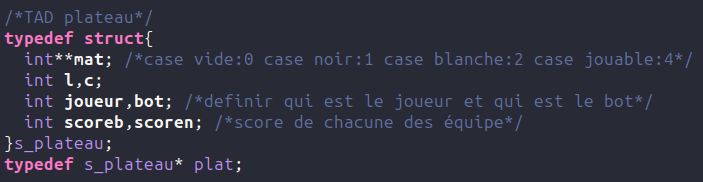
\includegraphics[scale=0.4]{fich/struct_plateau.png}
\end{frame}

\subsection{Structure arbre}
\begin{frame}
  \frametitle{Structure arbre}
  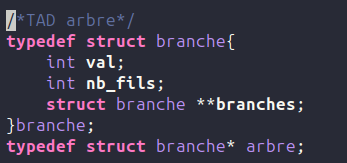
\includegraphics[scale=0.4]{fich/struct_arbre.png}
\end{frame}

\subsection{Structure coordonnées}
\begin{frame}
  \frametitle{Structure coordonnée}
  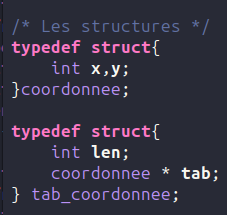
\includegraphics[scale=0.4]{fich/struct_coordonnees.png}
\end{frame}

\section{Difficultées rencontrées}
\begin{frame}
  \frametitle{Difficultés rencontrées}
\end{frame}

\section{Solution trouvées}
\begin{frame}
  \frametitle{Solutions trouvées}
\end{frame}

\section{Difficultées non résolues}
\begin{frame}
  \frametitle{Difficultés non résolues}
\end{frame}

\section{Conclusion}
\begin{frame}
  \frametitle{Conclusion}
  Merci de votre attention
\end{frame}

\end{document}
